\documentclass[12pt]{article}
\usepackage{geometry}                % See geometry.pdf to learn the layout options. There are lots.
\geometry{letterpaper}                   % ... or a4paper or a5paper or ... 
%\geometry{landscape}                % Activate for for rotated page geometry
\usepackage[parfill]{parskip}    % Activate to begin paragraphs with an empty line rather than an indent
\usepackage{daves,fancyhdr,natbib,graphicx,dcolumn,amsmath,lastpage,url}
\usepackage{amsmath,amssymb,epstopdf,longtable}
\usepackage[final]{pdfpages}
\DeclareGraphicsRule{.tif}{png}{.png}{`convert #1 `dirname #1`/`basename #1 .tif`.png}
\pagestyle{fancy}
\lhead{CE 3354 -- Engineering Hydrology}
\rhead{SUMMER 2025}
\lfoot{ES8}
\cfoot{}
\rfoot{Page \thepage\ of \pageref{LastPage}}
\renewcommand\headrulewidth{0pt}



\begin{document}
\begin{center}
{\textbf{{ CE 3354 Engineering Hydrology} \\ {Exercise Set 8}}}
\end{center}

\textbf{Scroll to bottom for a minimal solution sketch}

\section*{\small{Exercises}}
\begin{enumerate}

\item Figure \ref{fig:HardinCreekLayout} is a modeling layout for a HEC-HMS analysis of the US-84 crossing (lower right corner of the image).

\begin{figure}[h!] %  figure placement: here, top, bottom, or page
   \centering
   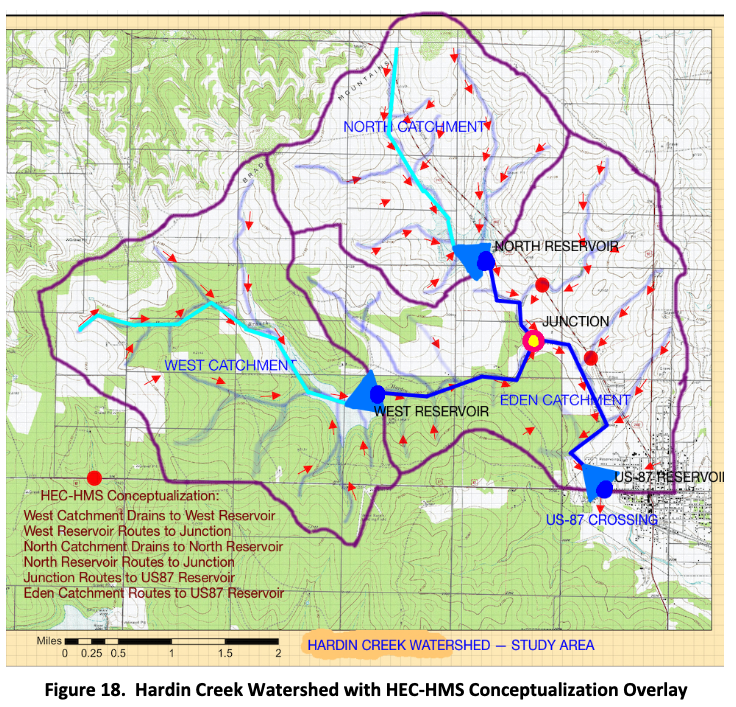
\includegraphics[height=6in]{HardinCreekLayout.png} 
   \caption{HEC-HMS Configuration for Hardin Creek Analysis}
   \label{fig:HardinCreekLayout}
\end{figure}

\clearpage

Supporting data are:

\begin{table}[h!]
\centering
\caption{Unit Hydrograph Parameters for 3 Catchments}
\begin{tabular}{p{1.0in}p{1.0in}p{1.0in}p{0.7in}p{0.7in}p{1.6in}} % Column formatting, @{} suppresses leading/trailing space
~&~\\
Name & Area (sq.mi.) & Length (mi) & Slope & T$_c$ (hrs) & Basin Lag (hrs)\\
\hline
\hline
North & 3.83& 2.74& 0.006& 5.19& 3.11\\
West & 6.04& 3.44& 0.004& 7.98& 4.78\\
Eden & 6.95& 3.69& 0.005& 4.76& 2.85\\
\hline
\end{tabular}
\label{tab:UH_hardin}
\end{table}

\begin{table}[h!]
\centering
\caption{Elevation-Area for North Reservoir}
\begin{tabular}{p{2.0in}p{2.0in}} % Column formatting, @{} suppresses leading/trailing space
~&~\\
Pool Elevation (ft) & Surface Area (acres) \\
\hline
\hline
2055 & 0.0\\
2065 & 61.44\\
2070 & 115.2\\
2076 & 192.0\\
\hline
\end{tabular}
\label{tab:EA_North}
\end{table}

\begin{table}[h!]
\centering
\caption{Elevation-Area for West Reservoir}
\begin{tabular}{p{2.0in}p{2.0in}} % Column formatting, @{} suppresses leading/trailing space
~&~\\
Pool Elevation (ft) & Surface Area (acres) \\
\hline
\hline
2065 & 0.0\\
2075 & 115.20\\
2080 & 235.52\\
2087 & 329.60\\
\hline
\end{tabular}
\label{tab:EA_West}
\end{table}

The outlet(s) for the North and West Reservoirs are 4-foot diameter orifices that activate at 10 feet above the dam base (empty pool) elevation.  These drain into the streams on the downstream side of each dam.

\begin{table}[h!]
\centering
\caption{Elevation-Area for US-87 (Upstream Side of Culverts) as a Reservoir}
\begin{tabular}{p{2.0in}p{2.0in}} % Column formatting, @{} suppresses leading/trailing space
~&~\\
Pool Elevation (ft) & Surface Area (acres) \\
\hline
\hline
2010 & 0.0\\
2020 & 3.29\\
2030 & 115.2\\
\hline
\end{tabular}
\label{tab:EA_87}
\end{table}

\clearpage

Figure \ref{fig:2barrel} is a cross-section view looking downstream at the US-87 Crossing (US-87
Reservoir Outlet) with the existing 2-barrel system depicted. The road profile is the grey
region that slopes down to the top of the culverts then back up.

\begin{figure}[h!] %  figure placement: here, top, bottom, or page
   \centering
   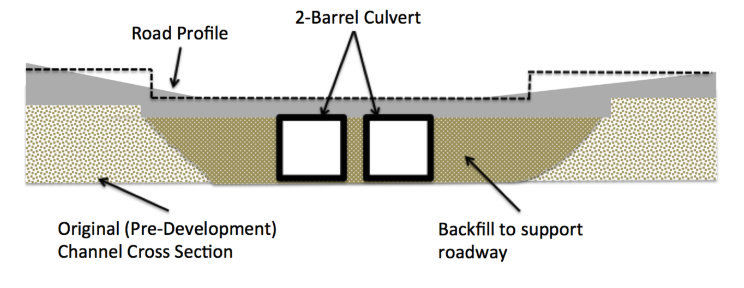
\includegraphics[width=6in]{2barrel.png} 
   \caption{2-Barrel Culvert configuration at US-87}
   \label{fig:2barrel}
\end{figure}

Figure \ref{fig:4barrel} is s cross-section view looking downstream at the US-87 Crossing (US-87
Reservoir Outlet) with the proposed 4-barrel system depicted.

\begin{figure}[h!] %  figure placement: here, top, bottom, or page
   \centering
   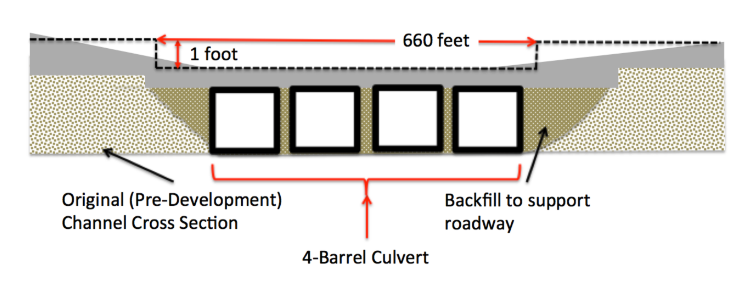
\includegraphics[width=6in]{4barrel.png} 
   \caption{4-Barrel Culvert configuration at US-87}
   \label{fig:4barrel}
\end{figure}

\newpage
Figure \ref{fig:Culvert Profile} is a side–view of the roadway crossing showing the embankment and the
culvert system, along with the elevations of the upstream end of the culvert, the top of
the culvert, and the roadway elevation.

\begin{figure}[h!] %  figure placement: here, top, bottom, or page
   \centering
   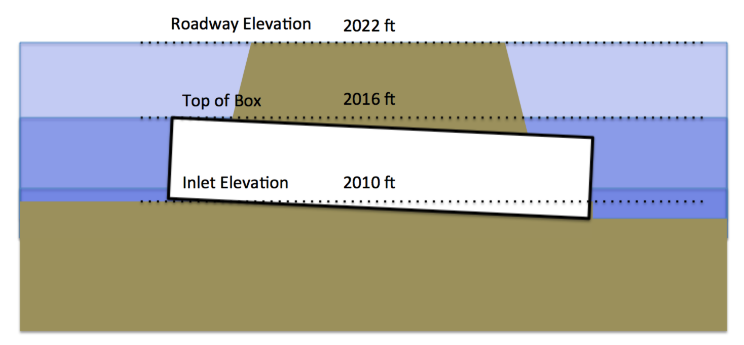
\includegraphics[width=6in]{CulvertProfile.png} 
   \caption{Culvert profile at US-87}
   \label{fig:Culvert Profile}
\end{figure}

\clearpage

The cross section for the channel connecting the outlet of the North Reservoir to the Junction is shown on Figure \ref{fig:CS_North}. The channel is a grass-lined
channel; Manning’s $n$ for the section is 0.035. The average channel slope is 0.6-percent. The length of the channel is 6020 feet.

\begin{figure}[h!] %  figure placement: here, top, bottom, or page
   \centering
   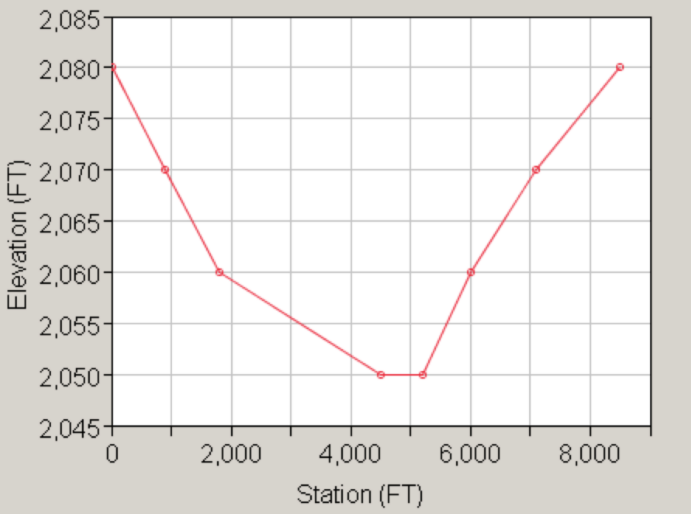
\includegraphics[width=6in]{CS_North.png} 
   \caption{Cross Section North to Junction (Typical)}
   \label{fig:CS_North}
\end{figure}

\clearpage

The cross section for the channel connecting the outlet of the West Reservoir to the Junction is shown on Figure \ref{fig:CS_West}. The channel is a grass-lined
channel; Manning’s $n$ for the section is 0.035. The average channel slope is 0.4-percent. The length of the channel is 8395 feet.

\begin{figure}[h!] %  figure placement: here, top, bottom, or page
   \centering
   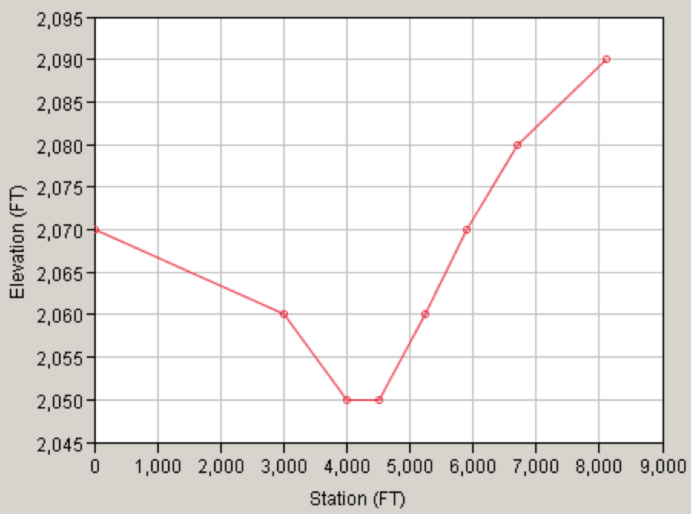
\includegraphics[width=6in]{CS_West.png} 
   \caption{Cross Section West to Junction (Typical)}
   \label{fig:CS_West}
\end{figure}

\clearpage

The cross section for the channel connecting the Junction to the US-87 Forebay is shown on Figure \ref{fig:CS_Junction}. The channel is a grass-lined
channel; Manning’s $n$ for the section is 0.035. The average channel slope is 0.5-percent. The length of the channel is 9695 feet.

\begin{figure}[h!] %  figure placement: here, top, bottom, or page
   \centering
   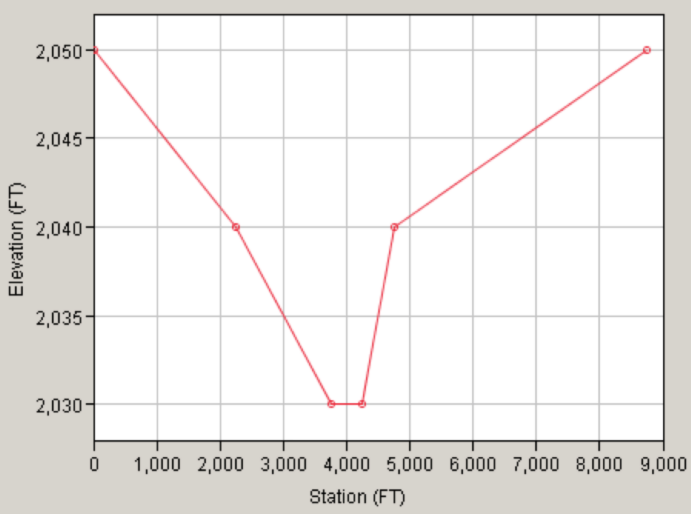
\includegraphics[width=6in]{CS_Junction.png} 
   \caption{Cross Section Junction to US-87(Typical)}
   \label{fig:CS_Junction}
\end{figure}

\clearpage

\textbf{Tasks}
Construct a HEC-HMS model using the supplied configuration. Use an NRCS Type-II storm distribution, to apply a 24-hour, 50-yr ARI design storm to the watershed.

Determine:
\begin{enumerate}
\item Determine the peak water surface elevation at the US-87 crossing when the two-barrel system is in place.
\item Determine the peak water surface elevation at the US-87 crossing when the four-barrel system is in place.
\end{enumerate}

\textbf{Deliverables}
\begin{enumerate}
\item A modeling report that shows the model output as hydrographs at US-87 under the different culvert systems, and
\item Model output showing the water depth in the US-87 Reservoir under the two conditions, and
\item Recomendation if culvert upgrade is needed.
\end{enumerate}

\end{enumerate}


\clearpage

\section*{\small{Solution}}

The HEC-HMS model was constructed using the supplied data.  The culvert system was conceptualized as 8 X 8 concrete box culverts (initially a pair, then a 4-barrel system).  The outlet structures method for the US87 reservoir was used, and the barrel count was changed to implement the two cases.

NOAA Atlas 14 Vol. 11 was consulted to find the 50-yr, 24-hr point depth near Eden Texas.  The value of 7.46 is used in the simulation(s).  Figure \ref{fig:pointdepth} is a screen capture of the relevant portion of the NOAA Atlas.

\begin{figure}[h!] %  figure placement: here, top, bottom, or page
   \centering
   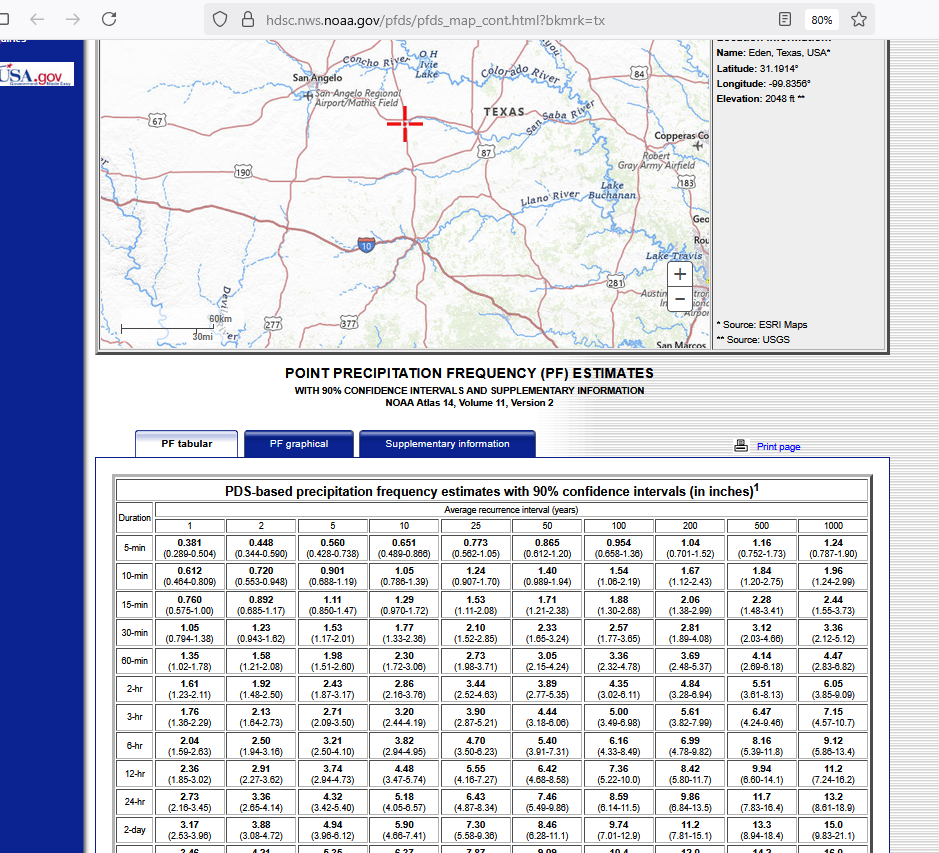
\includegraphics[width=6in]{pointdepth.png} 
   \caption{NOAA PFDS Screen Capture}
   \label{fig:pointdepth}
\end{figure}

The CN value for the North and West basin were set at 66 (which is probably high for the conditions); for the Eden basin which is about 30-percent developed a value of 87 was employed.

The Muskingum-Cunge method for routing was used based on the 3 supplied cross sections.  The Junction to US87 cross section was modified to have 8-points as required by the software - otherwise the values supplied ewre used.  The index flows wewe adjusted to obtain an index celerity of 1.0+ ft/second (target would be 1.46 ft/sec).  Any non-zero value would get the software to run.

The target pool elevation at US87 is 2022 feet, this is the modeled road elevation - pool elevation above this value means the simulation is predicting flow over the travel path.  

Figure \ref{fig:2X8by8BoxCulverts} is a screen capture of HEC-HMS run with the two-barrel system in place.

\begin{figure}[h!] %  figure placement: here, top, bottom, or page
   \centering
   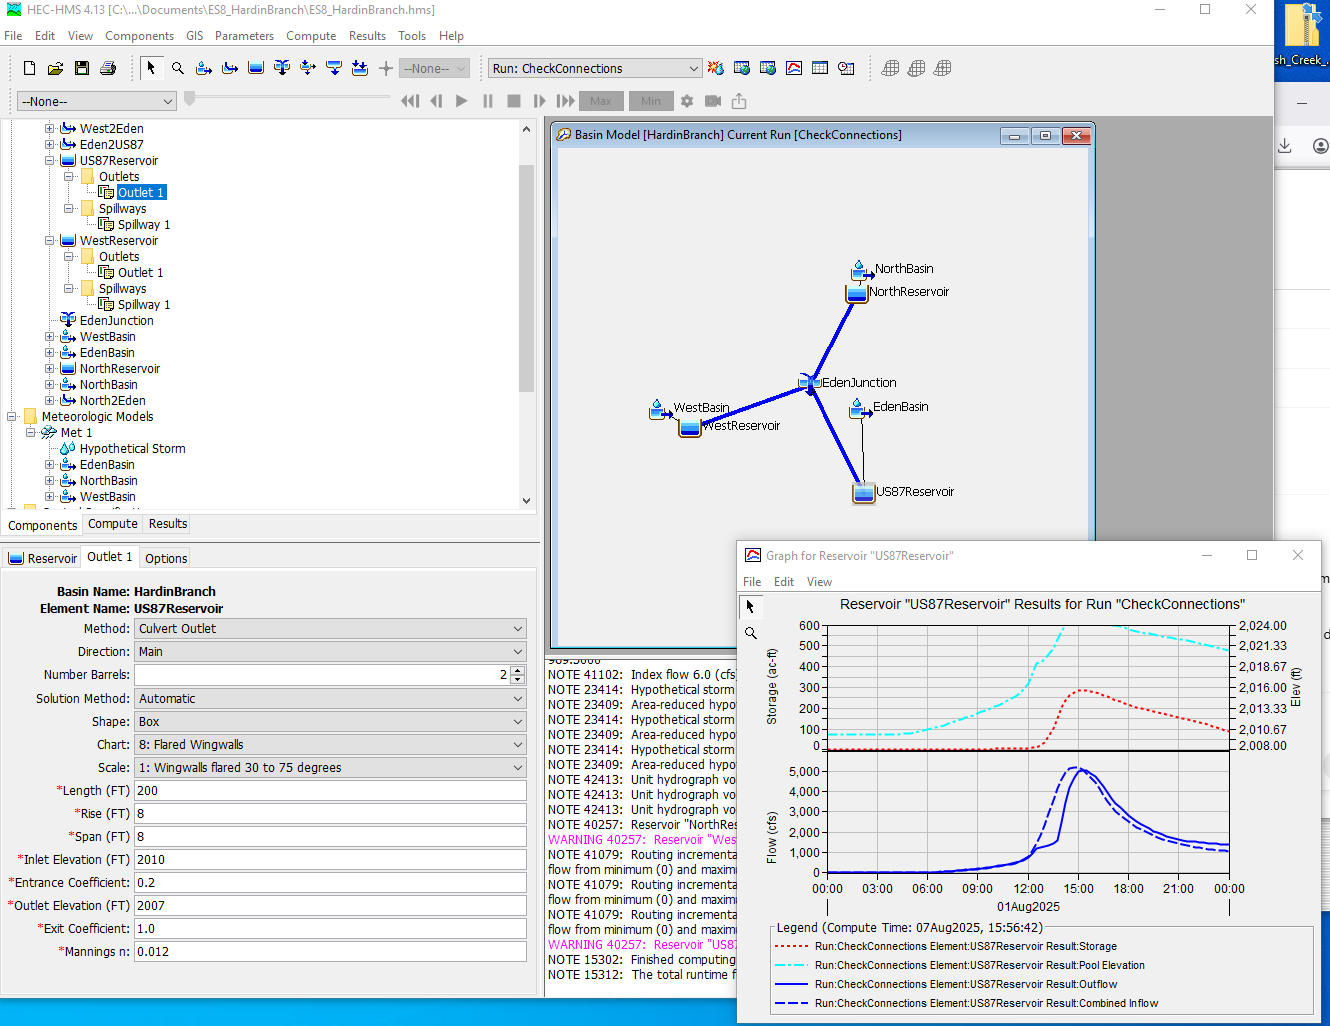
\includegraphics[width=6in]{2X8by8BoxCulverts.png} 
   \caption{HEC-HMS run for 2-barrel box at US-87; Pool elevation is 2024.5 ft, which is above the roadway elevation, therefore travel path is submerged.}
   \label{fig:2X8by8BoxCulverts}
\end{figure}

\clearpage

Figure \ref{fig:4X8by8BoxCulverts} is a screen capture of HEC-HMS run with the two-barrel system in place.

\begin{figure}[h!] %  figure placement: here, top, bottom, or page
   \centering
   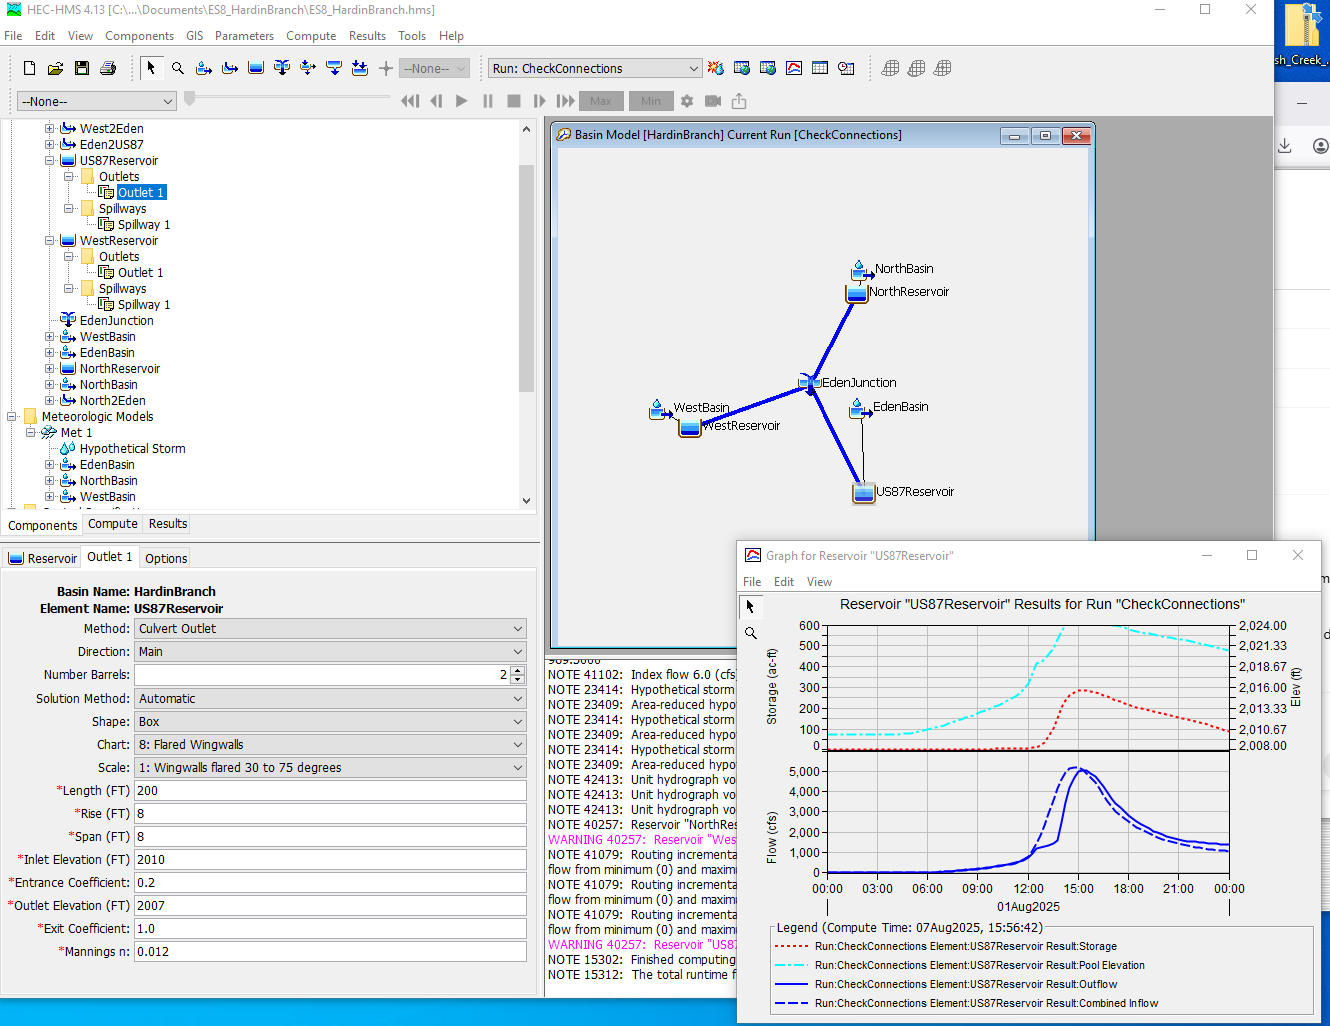
\includegraphics[width=6in]{2X8by8BoxCulverts.png} 
   \caption{HEC-HMS run for 2-barrel box at US-87; Pool elevation is 2023 ft, which is above the roadway elevation, therefore travel path is submerged.}
   \label{fig:4X8by8BoxCulverts}
\end{figure}

\clearpage

An addition of a 5-th and 6-th barrel, achieves an acceptable pool elevation at the US 87 location, albeit with only 1-inch of freeboard, nevertheless the simulation provides a starting point for design of a hydraulic structure to convey the flow beneath the roadway.

Figure \ref{fig:6X8by8BoxCulverts} is a screen capture of HEC-HMS run with the six-barrel system in place.

\begin{figure}[h!] %  figure placement: here, top, bottom, or page
   \centering
   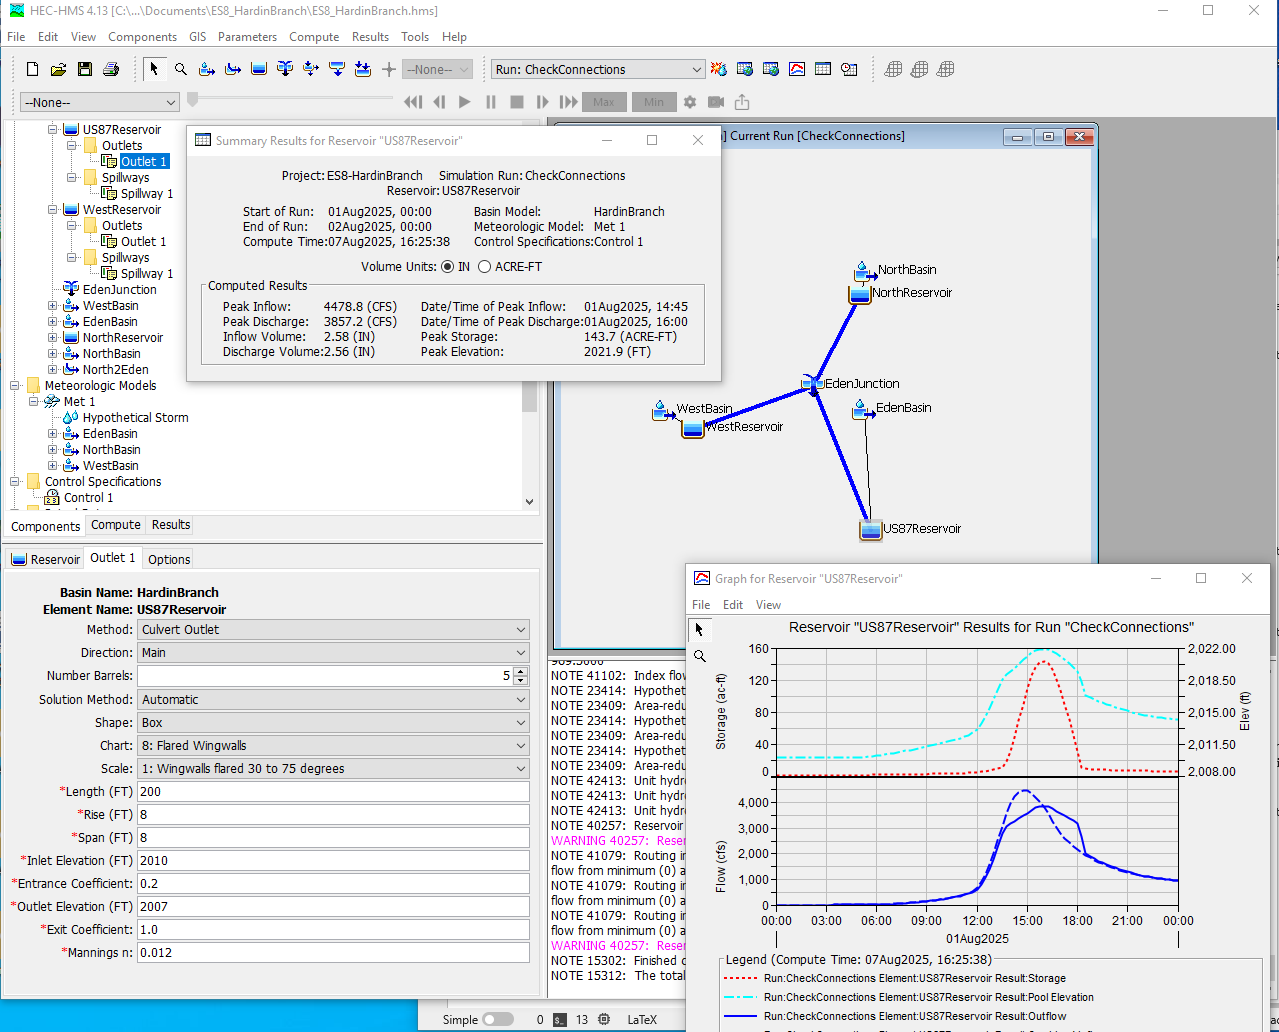
\includegraphics[width=6in]{6X8by8BoxCulverts.png} 
   \caption{HEC-HMS run for 6-barrel box at US-87; Pool elevation is 2021.9 ft, which is just below the roadway elevation, therefore travel path is unimpacted.}
   \label{fig:6X8by8BoxCulverts}
\end{figure}

The HEC-HMS project is stored at \url{http://54.243.252.9/ce-3354-webroot/hydrohandbook/exercises/08-hydrologicmodels/ES8_HardinBranch.zip}


\end{document}  